\documentclass[10pt, conference]{IEEEtran}
\IEEEoverridecommandlockouts
% The preceding line is only needed to identify funding in the first footnote. If that is unneeded, please comment it out.
\usepackage{cite}
\usepackage{amsmath,amssymb,amsfonts}
% \usepackage{algorithmic}
\usepackage{graphicx, wrapfig, subcaption}
\usepackage{textcomp}
\usepackage{xcolor}
\usepackage[numbers]{natbib} % Manual of natbib at https://gking.harvard.edu/files/natnotes2.pdf
\usepackage[hidelinks]{hyperref}
\usepackage[OT1]{fontenc} 
\begin{document}

\title{Conference Paper Title*\\
{\small CS494 - Wearable Technologies $\mid$ Professor Esmailbeigi}
% \thanks{Identify applicable funding agency here. If none, delete this.}
}

\author{\IEEEauthorblockN{Davide Giacomini}
\IEEEauthorblockA{\textit{dept. of Engineering} \\
\textit{University of Illinois at Chicago (UIC)}\\
Chicago (IL), USA \\
giacomini.davide@outlook.com}
\\
\IEEEauthorblockN{Jake Campbell}
\IEEEauthorblockA{\textit{dept. of Engineering} \\
\textit{University of Illinois at Chicago (UIC)}\\
Chicago (IL), USA \\
jacobpmcampbell@gmail.com}
\and
\IEEEauthorblockN{Sem Belay}
\IEEEauthorblockA{\textit{dept. of Engineering} \\
\textit{University of Illinois at Chicago (UIC)}\\
Chicago (IL), USA \\
sbelay2@uic.edu}
\\
\IEEEauthorblockN{Alejandro Dorvall}
\IEEEauthorblockA{\textit{dept. of Engineering} \\
\textit{University of Illinois at Chicago (UIC)}\\
Chicago (IL), USA \\
adorva2@uic.edu}
% \and
% \IEEEauthorblockN{5\textsuperscript{th} Given Name Surname}
% \IEEEauthorblockA{\textit{dept. name of organization (of Aff.)} \\
% \textit{name of organization (of Aff.)}\\
% City, Country \\
% email address or ORCID}
% \and
% \IEEEauthorblockN{6\textsuperscript{th} Given Name Surname}
% \IEEEauthorblockA{\textit{dept. name of organization (of Aff.)} \\
% \textit{name of organization (of Aff.)}\\
% City, Country \\
% email address or ORCID}
}

\maketitle
\thispagestyle{plain}
\pagestyle{plain}

\begin{abstract}
    In the current state of the pandemic, local clinics have become more important than ever. We will present a glove with an embedded display which can rapidly detect Covid-19 related symptoms by touching the patient.
\end{abstract}

\begin{IEEEkeywords}
TODO: insert words
\end{IEEEkeywords}

\section{Introduction}
In the pandemic era of SARS covid 19, there have been multiple ways in identifying  the viral disease. There have been many identification methods that include tracking symptoms and using built testing methods such as PCR \cite{smyrlaki2020massive}. These methods are known to be feasible and used to identify symptoms. Interestingly, on a regular  level it has been seen that clinics check for oxygen and temperature levels when examining patients for the viral disease. This method ensures if patients are more likely susceptible to the disease or if they are in the clear. It is known from studies that a patient with a temperature greater than or equal to 37.8 degree celsius is more likely at risk of coronavirus disease \cite{jang2020prognostic}. Also, it is a known fact that an oxygen saturation below 92\% is a potential risk of covid 19 disease \cite{jang2020prognostic}. This information gives clinical workers the basic information to assess a patient's risk of coronavirus. Unluckily, the interaction of clinic workers with patients involves direct contact. Some of these safety measures have come at the cost of efficiency. Our proposal is to design a solution for this issue. In the project we try to implement the same concept of using temperature and oxygen saturation to identify patients' risk by limiting the amount of contact. Our design is a glove with a temperature and pulse monitoring sensor built into the fingers as well as an LCD screen that sits on the back of the clinic worker’s hand. This will allow the worker to quickly hold the sensors to the patient’s wrist and finger, while running other diagnostics, and the device will output the data to the LCD screen as well as present a suggested Covid-19 diagnosis. The device will also have a wireless optional companion user interface that is run on a computer. The interface will display a review of the data and diagnosis from the gloves, but also allow the clinic worker to see a live graph of the patient’s temperature and oxygen level. The temperature graphs will also be able to be preset to either Farenhiet, Celsius, or Kelvin. Having stated the need statement it is important to consider the sensors and equipment that are able to make this possible. 

To measure oxygen saturation we use an oximeter sensor known as the Photoplethysmography (PPG)\footnote{\href{https://www.sparkfun.com/products/15219}{https://www.sparkfun.com/products/15219}}(Figure \ref{fig:oximeter}). This sensor is a pulse rate sensor that is mainly found in smart fitbit watches with a component having a light-emitting diode (LED) and a photodetector (PD) for measuring changes in light absorption. The sensor takes in the measurement of oxygen from the wrist since heart pulses are detected from there. It is important to note that the sensor that is used is a SparkFun module and is assembled to a peripheral board as such. When considering a temperature sensor, we wanted limited contact, which was achieved by using an infrared ray that can read temperature from a range . The sensor used is known as IR Thermometer Evaluation Board - MLX90614\footnote{\href{https://www.sparkfun.com/products/10740}{https://www.sparkfun.com/products/10740}}(Figure \ref{fig:thermometer}). This sensor is known for the high precision, small size, single zone IR thermometer with an optional SMBus (two-wire) or PWM interface. This gives us a temperature reading accurate enough to report human body temperature. The last equipment we wanted to incorporate was the Liquid Crystal Display (LCD) in the device. LCD’s are cheap and popular when it comes to displaying information such as sensor data. This will allow us to display the temperature and oxygen saturation on the device. With the power of a central board and peripheral board, we were able to combine these different sensors to make a wearable covid 19 testing device.

\begin{figure*}[t]
    \centering
    \begin{subfigure}[b]{.3\linewidth}
        \centering
        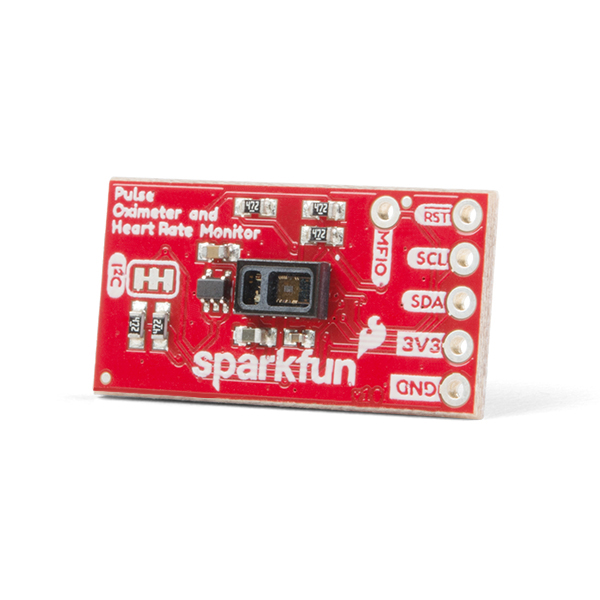
\includegraphics[width=\linewidth]{resources/oximeter.jpg}
        \caption{PPG sensor}
        \label{fig:oximeter}
    \end{subfigure}%
    \begin{subfigure}[b]{.3\linewidth}
        \centering
        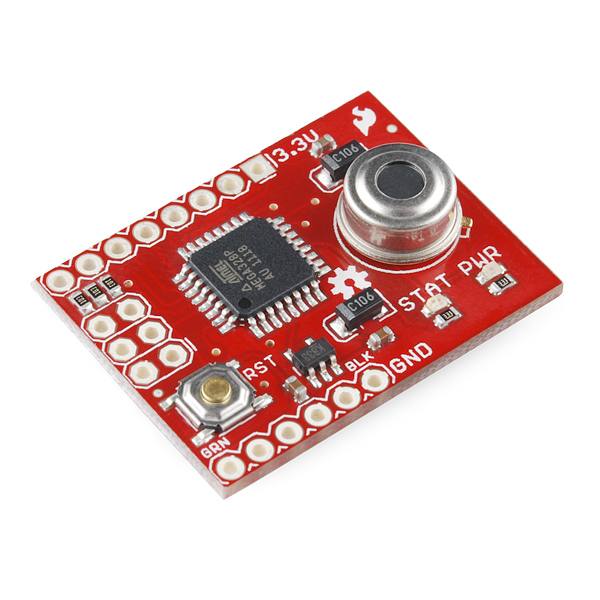
\includegraphics[width=\linewidth]{resources/thermoeter.jpg}
        \caption{MLX90614 sensor}
        \label{fig:thermometer}
    \end{subfigure}%
    \begin{subfigure}[b]{.3\linewidth}
        \centering
        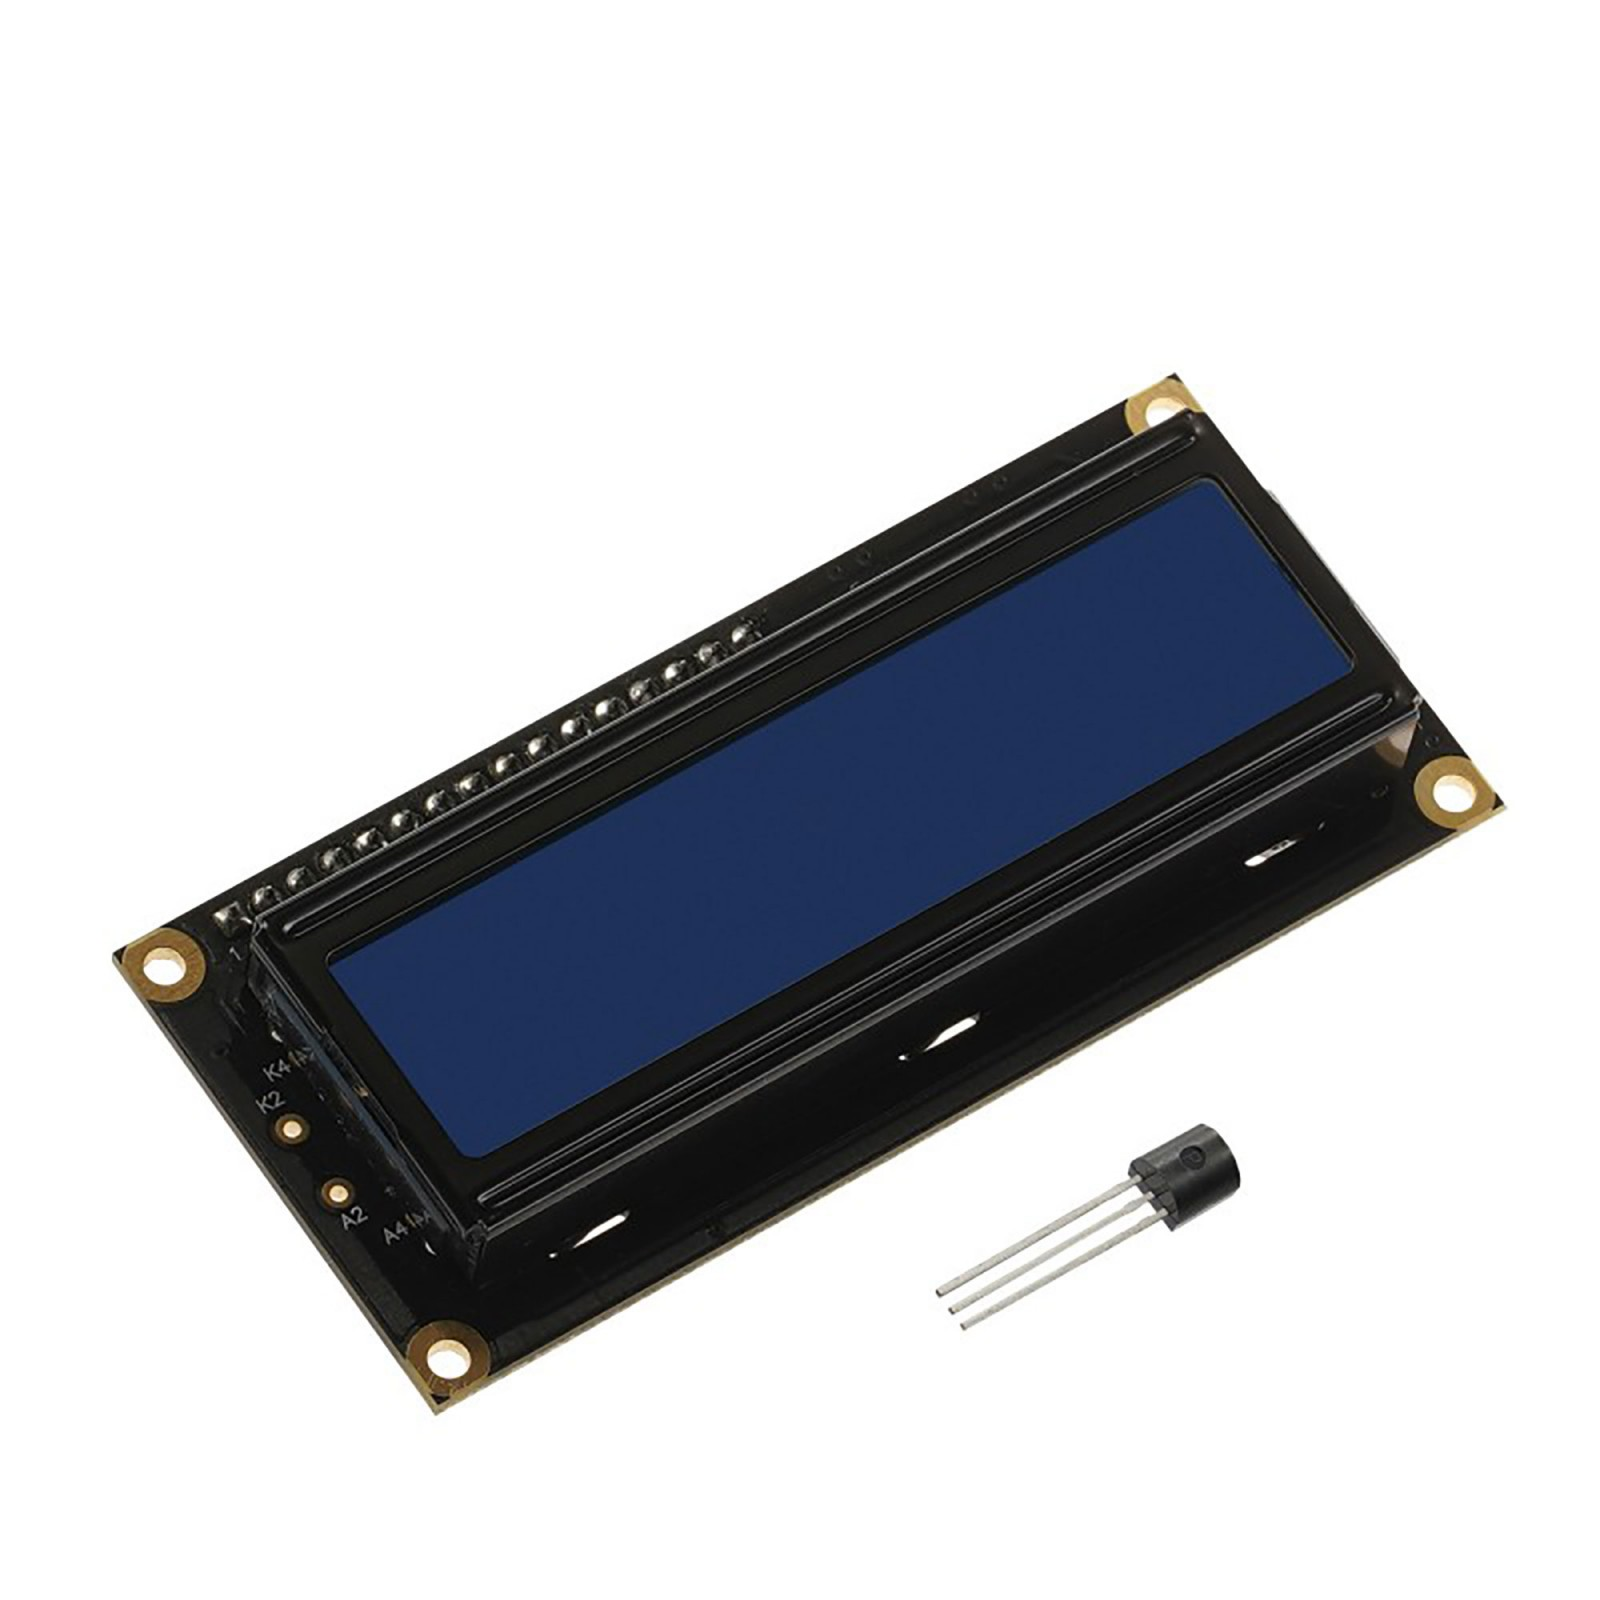
\includegraphics[width=\linewidth]{resources/LCD.jpg}
        \caption{LCD sensor}
        \label{fig:LCD}
    \end{subfigure}
    \label{fig:sensors}
    \caption{Sensors used for the device}
\end{figure*}

\section{Method}
\begin{figure*}[t]
    \centering
    \begin{subfigure}[b]{.3\linewidth}
        \centering
        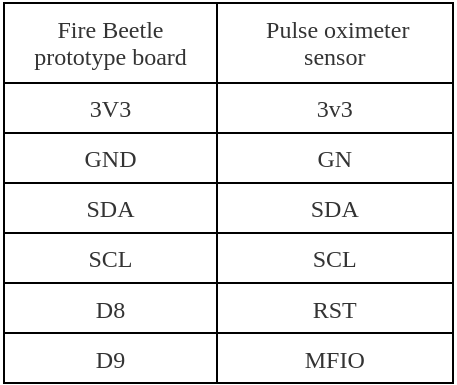
\includegraphics[width=.9\linewidth]{resources/pin-connections-oximeter.png}
        \caption{Oximeter pins}
        \label{fig:pin-oximeter}
    \end{subfigure}%
    \begin{subfigure}[b]{.3\linewidth}
        \centering
        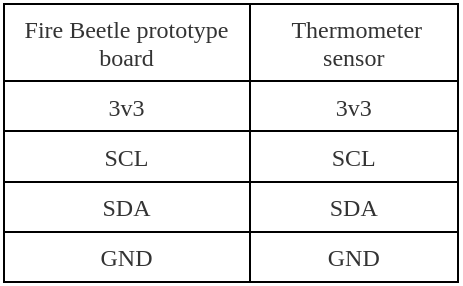
\includegraphics[width=.9\linewidth]{resources/pin-therm.png}
        \caption{Thermometer pins}
        \label{fig:pin-therm}
    \end{subfigure}%
    \begin{subfigure}[b]{.3\linewidth}
        \centering
        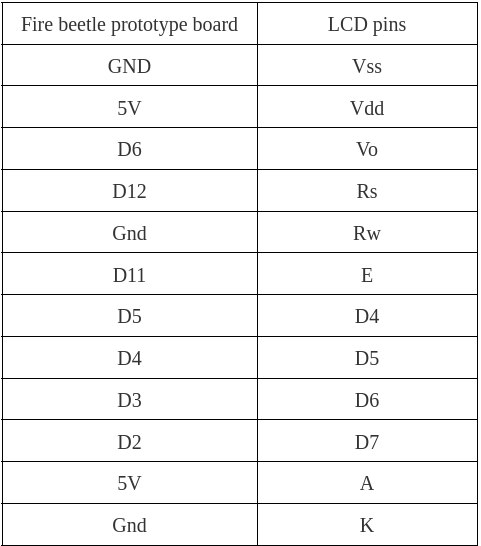
\includegraphics[width=.9\linewidth]{resources/pin-lcd.png}
        \caption{LCD pins}
        \label{fig:pin-lcd}
    \end{subfigure}
    \label{fig:pins}
    \caption{Pin connections for our devices}
\end{figure*}
The build of the device required a central board, peripheral board, and a prototype board. The prototype board will require pins to be soldered in so that it can be attached to the peripheral board. We will incorporate the two sensors and LED on the peripheral board. The pins incorporated have to be maneuvered by color coding since all the pins on the prototype board are used. Starting with the pulse sensor, we need to first ground and add a 3v3 voltage for power which is achieved by having it connected to the corresponding pins on the peripheral board. Having done that, we want the SCL and SDA for the pulse sensor connected to the prototype board. The SDA and SCL pin of the sensor is wire wrapped to the same corresponding pin of the prototype board. Interestingly, the pins left from the pulse sensor are RST and the MFIO which will be wire wrapped to the D8 and D9 pins of the peripheral board. The corresponding pin layout for the pulse sensor are shown at figure \ref{fig:pin-oximeter}.

Having connected the pulse sensor, we move on and connect the thermometer on the same peripheral board. It is important to note that the same pins cannot be used for connection on the prototype board. This is because the signals will interfere with each other causing the device to lose functionality. The only pins we can connect to similar pins are the power 3v3 and GND pins. Another interesting fact is that the thermometer pins also need connection to the SDA and SCL pins. This can be achieved by having different addresses when implementing code for the pulse and thermometer sensor. The pin connection for the thermometer are shown at figure \ref{fig:pin-therm}.

Having this connection on the board  will give us all the necessary value to make the predictions if a patient has covid 19. As the last design scheme, an LCD connection with these sensors will give a visual representation of a patient's diagnosis. The LCD pin connections involve more wiring than both the sensors. Also, it  requires a 5 V range that is replaced by a VCC pin on the prototype board and requires most of the digital pins of the prototype board to be wired wrapped with the LCD pins. The exact pin connections between the boards are shown at figure \ref{fig:pin-lcd}.

After having the connections, the next cycle involves the actual glove design. For this design we attach the pulse meter to the index finger of the gloves. This makes it easy for the user to measure oxygen saturation for the patient while keeping a necessary distance. The oxygen level will be measured from the patient's index finger as well. The temperature sensor will be placed on the middle finger of the glove. This gives the accessibility to measure the temperature with comfortability for both the user and patient. Information is processed and shown on the top side view of the gloves by the LCD screen. This makes information easy to view for the user and diagnose the patient accordingly. 


\bibliographystyle{unsrtnat} % Cannot upload \bibliographystyle{IEEEtran}, don't know why
\bibliography{bibliography}

\end{document}
